\documentclass[8pt,ignorenonframetext,]{beamer}
\usetheme{CambridgeUS}
\usecolortheme{beaver}
\usepackage{amssymb,amsmath}
\usepackage{xcolor}
%\usepackage{listings}
\usepackage[spanish,activeacute]{babel}
\usepackage[utf8]{inputenc}
% \usepackage{ifxetex,ifluatex}
% \ifxetex
  % \usepackage{fontspec,xltxtra,xunicode}
  % \defaultfontfeatures{Mapping=tex-text,Scale=MatchLowercase}
% \else
  % \ifluatex
    % \usepackage{fontspec}
    % \defaultfontfeatures{Mapping=tex-text,Scale=MatchLowercase}
  % \else
    % \usepackage[utf8]{inputenc}
  % \fi
% \fi
\usepackage{listings}
\lstnewenvironment{codeH}{\lstset{language=Haskell,basicstyle=\tiny\ttfamily,backgroundcolor=\color{green}}}{}
\lstnewenvironment{codeR}{\lstset{language=R,basicstyle=\tiny\ttfamily,backgroundcolor=\color{green}}}{}
\definecolor{lightgray}{gray}{.9}
\definecolor{mediumgray}{gray}{.6}
\lstset{
  literate={á}{{\'a}}1
           {é}{{\'e}}1
           {í}{{\'i}}1
           {ó}{{\'o}}1
           {ú}{{\'u}}1
           {ñ}{{\~n}}1
           {¿}{{?`}}1
}
\lstset{language=R,basicstyle=\tiny\ttfamily,backgroundcolor=\color{lightgray},showstringspaces=false}
\usepackage{ctable}
\usepackage{float} % provides the H option for float placement
\usepackage{url}
% Comment these out if you don't want a slide with just the
% part/section/subsection/subsubsection title:
\AtBeginPart{\frame{\partpage}}
\AtBeginSection{\frame{\sectionpage}}
\AtBeginSubsection{\frame{\subsectionpage}}
\AtBeginSubsubsection{\frame{\subsubsectionpage}}
% \setlength{\parindent}{0pt}
% \setlength{\parskip}{6pt plus 2pt minus 1pt}
% \setlength{\emergencystretch}{3em}  % prevent overfull lines
\setcounter{secnumdepth}{0}

\title{La librería ggplot2}
\author{Carlos Pérez Glez.}
\institute[Universidad de La Laguna]{
Universidad de La Laguna\\
Fundación General Universidad de La Laguna\\
Instituto Canario de Estadística
}
\setbeamertemplate{navigation symbols}{}

\date{}

      
\begin{document}
\frame{\titlepage}

\begin{frame}\frametitle{La librería ggplot2}

\begin{enumerate}
\def\labelenumi{\arabic{enumi}.}
\itemsep1pt\parskip0pt\parsep0pt
\item
  Es un paquete que permite generar gráficos estadísticos.
\item
  Se diferencia de otras librerías en el aspecto de controlar una gran
  número de componentes gráficos (``gramática de gráficos'').
\item
  Los gráficos se pueden construir añadiéndole sucesivamente más
  atributos o capas (``layers'').\\ Libro: H.Wickham (2009). ggplot2:
  Elegant Graphics for Data Analysis 123, Use R!, Springer Website:
  http://had.co.nz/ggplot2 Tutorial:
  http://www.ceb-institute.org/bbs/wp-content/uploads/2011/09/handout\_ggplot2.pdf
\end{enumerate}

\end{frame}

\begin{frame}\frametitle{El comando qplot()}

\begin{center}
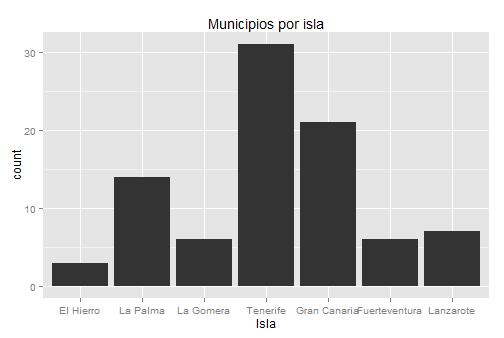
\includegraphics[width=0.4\textwidth]{figure/plot01.png}
\end{center}

Los comandos gráficos disponibles en ggplot2 son:

\begin{itemize}
\item
  qplot() - para ``quick plots''
\item
  ggplot() - para mejor ajuste y control de todo
\end{itemize}

\end{frame}

\begin{frame}[fragile]\frametitle{El comando qplot(): ejemplos}

Veamos algunos ejemplos:

\begin{lstlisting}[language=R]
qplot(data=data.geo.municipios,x=Superficie,main="Histograma de superficie",binwidth=50)

qplot(data=data.geo.islas,x=Superficie,y=Altitud, main="Gráfico de superficie vs. altitud")

qplot(data=data.geo.islas,x=Superficie,y=Altitud, main="Gráfico de superficie vs. altitud", 
xlab="Superficie de la isla", ylab="Altitud de la isla")

qplot(data=data.geo.islas,x=Superficie,y=Altitud, main="Gráfico de superficie vs. altitud", 
xlab="Superficie de la isla", ylab="Altitud de la isla",
xlim=c(0,2500),ylim=c(0,1500))
\end{lstlisting}

\end{frame}

\begin{frame}[fragile]\frametitle{Color, tamaño, forma (aspectos
estéticos)}

Con el comando clásico plot(), si queremos representar variables
categóricas (e.g.~una variable de tipo sexo, ``Hombre'',``Mujer'') con
colores, debemos realizar nosotros mismos la correspondencia entre
categoría y color.

En qplot() se puede especificar varios argumentos: colour, size, shape

\begin{lstlisting}[language=R]
qplot(data=data.geo.islas,x=Superficie,y=Altitud, colour = Isla,
main="Gráfico de superficie vs. altitud", 
xlab="Superficie", ylab="Altitud") 
\end{lstlisting}

\begin{lstlisting}[language=R]
qplot(data=data.geo.islas,x=Superficie,y=Altitud, size = Isla,
main="Gráfico de superficie vs. altitud", 
xlab="Superficie", ylab="Altitud") 
\end{lstlisting}

\begin{lstlisting}[language=R]
qplot(data=data.geo.islas,x=Superficie,y=Altitud, shape = Isla,
main="Gráfico de superficie vs. altitud", 
xlab="Superficie", ylab="Altitud") +
scale_shape_manual(values=1:7)
\end{lstlisting}

\end{frame}

\begin{frame}\frametitle{Objetos geométricos}

qplot no está limitado a gráficos de dispersión (scatterplot), sino que
puede producir casi cualquier tipo de gráfico variando el argumento
geom.

\begin{itemize}
\itemsep1pt\parskip0pt\parsep0pt
\item
  geom = ``point'' representa puntos para producir un scatterplot. Esta
  es la opción por defecto cuando se pasan argumentos x e y a qplot().
\item
  geom = ``boxplot'' produce un gráfico box-and-whisker plot de resumen
  de la distribución de un conjunto de puntos.
\item
  geom = ``smooth'' ajusta una curva suavizada a los datos (smoother) y
  su error estándar. Esta opción se combina con un argumento method
  \%in\% c(``loess'',``gam'',``lm'',``rlm'') (ver
  http://docs.ggplot2.org/0.9.3/stat\_smooth.html)
\item
  geom = ``path'' and geom = ``line'' representa lineas entre los
  puntos.
\end{itemize}

\end{frame}

\begin{frame}[fragile]\frametitle{Ejemplos de ggplot() - objetos
geométricos}

Vemos algunos ejemplos:

\begin{lstlisting}[language=R]
qplot(data=data.geo.municipios,x=Superficie,y=Altitud, geom = "point")

qplot(data=data.geo.municipios,x=Superficie,y=Altitud, geom = "boxplot", colour = Isla)    # cuidado con el tipo de variables
qplot(data=data.geo.municipios,x=Isla,y=Altitud, geom = "boxplot")

qplot(data=data.geo.municipios,x=Superficie,y=Altitud, geom = "smooth", method="loess")
qplot(data=data.geo.municipios,x=Superficie,y=Altitud, geom = c("point", "smooth"), method="lm")

qplot(data=data.geo.municipios,x=Superficie,y=Altitud, geom = "path")
qplot(data=data.geo.municipios,x=Superficie,y=Altitud, geom = "line")

qplot(data=data.geo.municipios, x=Provincia, geom = "bar")
qplot(data=data.geo.municipios, x=Superficie, geom = "histogram")
qplot(data=data.geo.municipios, x=Superficie, geom = "density")
\end{lstlisting}

\end{frame}

\begin{frame}[fragile]\frametitle{Comprensión de la gramática de capas}

\begin{enumerate}
\def\labelenumi{\arabic{enumi}.}
\item
  Podemos usar sólo qplot() pero la verdadera potencia de ggplot2 está
  en el manejo de los gráficos por capas (gramática de capas) mediante
  ggplot().
\item
  El qplot recorta bastantes detalles de ggplot() a pesar que permite
  una sintaxis más familiar y cercana al plot().
\item
  Con ggplot(), sin embargo, es posible incorporar a un gráfico
  diferentes niveles de detalle mediante sucesivas capas (layers).
\end{enumerate}

\begin{lstlisting}[language=R]
ggplot(data, mapping) +
layer( 
      geom = "",  
      stat = "",  
      position = "", ....  
      )
\end{lstlisting}

\end{frame}

\begin{frame}\frametitle{Otros objetos geométricos en ggplot2}

\begin{longtable}[c]{@{}ll@{}}
\hline\noalign{\medskip}
Name & Description
\\\noalign{\medskip}
\hline\noalign{\medskip}
abline & Line, specified by slope and intercept
\\\noalign{\medskip}
area & Area plots
\\\noalign{\medskip}
bar & Bars, rectangles with bases on y-axis
\\\noalign{\medskip}
boxplot & Box-and-whisker plot
\\\noalign{\medskip}
contour & Display contours of a 3d surface in 2d
\\\noalign{\medskip}
errorbar & Error bars
\\\noalign{\medskip}
histogram & Histogram
\\\noalign{\medskip}
line & Connect observations, in order of x value
\\\noalign{\medskip}
point & Points, as for a scatterplot
\\\noalign{\medskip}
polygon & Polygon, a filled path
\\\noalign{\medskip}
step & Connect observations by stairs
\\\noalign{\medskip}
text & Textual annotations
\\\noalign{\medskip}
\hline
\end{longtable}

\end{frame}

\begin{frame}\frametitle{Algunas transformaciones estadísticas en
ggplot2}

\begin{longtable}[c]{@{}ll@{}}
\hline\noalign{\medskip}
Name & Description
\\\noalign{\medskip}
\hline\noalign{\medskip}
bin & Bin data
\\\noalign{\medskip}
boxplot & Calculate components of box-and-whisker plot
\\\noalign{\medskip}
contour & Contours of 3d data
\\\noalign{\medskip}
density & Density estimation
\\\noalign{\medskip}
function & Superimpose a function
\\\noalign{\medskip}
identity & Don't transform data
\\\noalign{\medskip}
quantile & Continuous quantiles
\\\noalign{\medskip}
smooth & Add a smoother
\\\noalign{\medskip}
step & Create stair steps
\\\noalign{\medskip}
sum & Sum unique values. Useful for overplotting on scatterplots
\\\noalign{\medskip}
summary & Summarise y values at every unique x
\\\noalign{\medskip}
unique & Remove duplicates
\\\noalign{\medskip}
\hline
\end{longtable}

\end{frame}

\begin{frame}[fragile]\frametitle{Scatterplot en ggplot2}

Un scatterplot:

\begin{lstlisting}[language=R]
ejemplo1<-qplot(data=data.geo.municipios,x=Superficie,y=Altitud, colour = Isla)
\end{lstlisting}

se compone de (http://docs.ggplot2.org/current/index.html):

\begin{itemize}
\item
  Un conjunto de datos por defecto (data).
\item
  Una asignación de variables del conjunto de datos a atributos gráficos
  (aesthetics).
\end{itemize}

\begin{lstlisting}[language=R]
ejemplo1<-ggplot(data=data.geo.municipios, mapping=aes(x=Superficie,y=Altitud, colour=Isla))
\end{lstlisting}

\end{frame}

\begin{frame}[fragile]\frametitle{Scatterplot en ggplot2: layers}

Y de las siguientes capas o layers:

\begin{itemize}
\itemsep1pt\parskip0pt\parsep0pt
\item
  El tipo de objeto geométrico (punto, línea, barra, \ldots{}) utilizado
  para la representación (geom).
\end{itemize}

\begin{lstlisting}[language=R]
  ejemplo1 + layer(geom="point")  # o tambien: ejemplo1 + geom_point() 
\end{lstlisting}

\begin{itemize}
\itemsep1pt\parskip0pt\parsep0pt
\item
  Una transformación estadística (suma, densidad, boxplot,..) de los
  datos (stat).
\end{itemize}

\begin{lstlisting}[language=R]
  ejemplo1 + layer(geom="point", stat="identity" ) # o tambien: ejemplo1 + geom_point(stat="identity")  
# o tambien: ejemplo1 + geom_point()  
\end{lstlisting}

\begin{center}
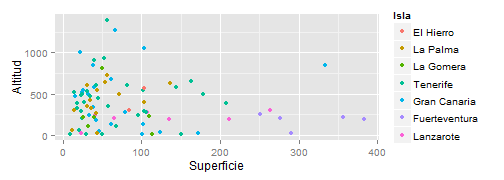
\includegraphics[width=0.4\textwidth]{figure/unnamed-chunk-6.png}
\end{center}

\end{frame}

\begin{frame}[fragile]\frametitle{Scatterplot en ggplot2: otros
aspectos}

Además, se puede

\begin{itemize}
\itemsep1pt\parskip0pt\parsep0pt
\item
  Controlar cómo se asignan las variables del conjunto de datos a los
  atributos aesthetics (scales). Por ejemplo, la forma (shape) o el
  tamaño (size) de los objetos puede cambiar según el valor de las
  variables.
\end{itemize}

\begin{lstlisting}[language=R]
  ejemplo1<-ggplot(data=data.geo.municipios, mapping=aes(x=Superficie,y=Altitud, colour=Isla))

  ejemplo1 + geom_point(mapping=aes(shape=Provincia) ) + scale_shape(solid = FALSE)  # cambiar la forma
  
  ejemplo1 + geom_point(mapping=aes(size=Provincia) ) + scale_size_discrete(range = c(2, 4) ) # cambiar el tamaño
\end{lstlisting}

\begin{itemize}
\itemsep1pt\parskip0pt\parsep0pt
\item
  Cambiar el sistema de representación de coordenadas (coord)
\end{itemize}

\begin{lstlisting}[language=R]
  ejemplo1 + geom_point() + coord_polar()
\end{lstlisting}

\begin{itemize}
\itemsep1pt\parskip0pt\parsep0pt
\item
  Especificar la visualización de subconjuntos de los datos en
  diferentes paneles (facet)
\end{itemize}

\begin{lstlisting}[language=R]
  ejemplo1 + geom_point() + facet_grid(. ~ Provincia)
\end{lstlisting}

\end{frame}

\begin{frame}[fragile]\frametitle{Gráfico de barras en ggplot2}

Un diagrama de barras:

\begin{lstlisting}[language=R]
ejemplo2<-qplot(data=data.geo.municipios,x=Provincia, geom = "bar", fill = Isla)
\end{lstlisting}

\begin{itemize}
\itemsep1pt\parskip0pt\parsep0pt
\item
  La asignación o mapping de variables (atributos aesthetics):
\end{itemize}

\begin{lstlisting}[language=R]
  ejemplo2<-ggplot(data=data.geo.municipios, mapping=aes(x=Provincia, fill=Isla))
\end{lstlisting}

\begin{itemize}
\itemsep1pt\parskip0pt\parsep0pt
\item
  El tipo de objeto geom:
\end{itemize}

\begin{lstlisting}[language=R]
  ejemplo2 + layer(geom="bar")    # o tambien: ejemplo2 + geom_bar()  
\end{lstlisting}

\end{frame}

\begin{frame}[fragile]\frametitle{Gráfico de barras en ggplot2: layers}

\begin{itemize}
\itemsep1pt\parskip0pt\parsep0pt
\item
  La transformación estadística stat:
\end{itemize}

\begin{lstlisting}[language=R]
  ejemplo2 + layer(geom="bar", stat="bin" )  
  # o tambien:  ejemplo2 + geom_bar(stat="bin")  
  # o tambien: ejemplo2 + geom_bar()
\end{lstlisting}

\begin{itemize}
\itemsep1pt\parskip0pt\parsep0pt
\item
  El ajuste de posición en el gráfico (position):
\end{itemize}

\begin{lstlisting}[language=R]
  ejemplo2 + layer(geom="bar", stat="bin", position="dodge")  
  # o tambien:  ejemplo2 + geom_bar(position=position_dodge() )   
\end{lstlisting}

\end{frame}

\begin{frame}[fragile]\frametitle{Otros gráficos en ggplot2}

Algunos ejemplos mas (densidad e histograma):

\begin{lstlisting}[language=R]
qplot(data=data.espacios.nat, x=Superficie, geom = "density", colour = Isla)   
# las densidades son superpuestas
 
ggplot(data=data.espacios.nat, mapping=aes(x=Superficie,colour=Isla)) +geom_density()
\end{lstlisting}

\begin{lstlisting}[language=R]
qplot(data=data.espacios.nat, x=Superficie, geom = "histogram", colour = Isla) 
# los histogramas son apilados y se colorea el borde

ggplot(data=data.espacios.nat, mapping=aes(x=Superficie,colour=Isla)) +geom_histogram()
\end{lstlisting}

\begin{lstlisting}[language=R]
qplot(data=data.espacios.nat, x=Superficie, geom = "histogram", fill = Isla)   
# los histogramas son apilados y se colorea el interior

ggplot(data=data.espacios.nat, mapping=aes(x=Superficie,fill=Isla)) +geom_histogram()
\end{lstlisting}

\end{frame}

\begin{frame}[fragile]\frametitle{Otros gráficos en ggplot2}

Algunos ejemplos mas (gráficos de barras):

\begin{lstlisting}[language=R]
qplot(data=data.espacios.nat, x=Espacio.natural, geom = "bar", fill = Isla) 
# también los gráficos de barras son apilados

ggplot(data=data.espacios.nat, mapping=aes(x=Espacio.natural,fill=Isla)) +geom_bar(position=position_dodge() )
\end{lstlisting}

\begin{lstlisting}[language=R]
qplot(data=data.espacios.nat, x=Espacio.natural, geom = "bar", fill = Isla, position="dodge") 
# barras colocadas unas al lado de otras

ggplot(data=data.espacios.nat, mapping=aes(x=Espacio.natural,fill=Isla)) +geom_bar()
\end{lstlisting}

\end{frame}

\begin{frame}[fragile]\frametitle{Otros gráficos en ggplot2}

Algunos ejemplos mas:

\begin{lstlisting}[language=R]
qplot(data=data.geo.municipios, x=Provincia, geom = "bar")

ggplot(data=data.geo.municipios, mapping=aes(x=Provincia)) +geom_bar()
\end{lstlisting}

\begin{lstlisting}[language=R]
qplot(data=data.geo.municipios, x=Provincia, geom = "bar", fill = Isla)

ggplot(data=data.geo.municipios, mapping=aes(x=Provincia,fill = Isla)) +geom_bar()
\end{lstlisting}

\end{frame}

\begin{frame}[fragile]\frametitle{Otros gráficos en ggplot2}

Algunos ejemplos mas:

\begin{lstlisting}[language=R]
qplot(data=data.geo.municipios, x=Superficie, geom = "histogram")

ggplot(data=data.geo.municipios, mapping=aes(x=Superficie) +geom_histogram()

qplot(data=data.geo.municipios, x=Superficie, geom = "density")

ggplot(data=data.geo.municipios, mapping=aes(x=Superficie) +geom_density()
       
qplot(data=data.geo.municipios, x=Superficie, geom = "density", colour = Provincia)   # las densidades son superpuestas

ggplot(data=data.geo.municipios, mapping=aes(x=Superficie, colour = Provincia)) +geom_density()
\end{lstlisting}

\end{frame}

\begin{frame}[fragile]\frametitle{Otros gráficos en ggplot2}

Algunos ejemplos mas:

\begin{lstlisting}[language=R]
qplot(data=data.geo.municipios, x=Superficie, geom = "histogram", colour = Provincia)  
# los histogramas son apilados y se colorea el borde
       
       
qplot(data=data.geo.municipios, x=Superficie, geom = "histogram", fill = Provincia)  
# los histogramas son apilados y se colorea el interior

qplot(data=data.geo.municipios, x=Superficie, geom = "histogram", fill = Provincia, position="dodge")  
# las barras se pueden representar sin apilar
       
\end{lstlisting}

\end{frame}

\end{document}
